\chapter{Discussion}

In this Chapter I will discuss how my results compare to others I have not yet touched upon and discuss their broader implications (Section~\ref{sec:bigpic}). I will also discuss the implications my results have for the proper use of morphology in galaxy evolution studies (Section~\ref{sec:usemorph}). I will then discuss future work with \starpy\ (Section~\ref{sec:future}) and its application to IFU spectral data (Section~\ref{sec:IFU}). I will end with a reflection on the power of Hubble Space Telescope imaging in comparison to SDSS imaging. 

\section{The Big Picture}\label{sec:bigpic}

In Chapter~\ref{chap:morph} I discussed how the results suggested that quenching rates with $\tau < 1.5~\rm{Gyr}$ must be caused by mechanisms which can transform morphology from a disc to an elliptical. However this does not infer an immediate transition from disc dominated to bulge dominated. Work by the \textsc{ATLAS}$^{\rm{3D}}$ team \citep{cappellari11} showed that kinematic discs are found in the majority of the visually elliptical population \citep{emsellem11} with $\sim7$ times the number of \emph{fast rotators} (with kinematic discs) than \emph{slow rotators} \citep[with dispersion dominated kinematics see][]{cappellari07, emsellem07}. 

The authors of these works discuss how dry major mergers, which can destroy the disk dominated nature of a galaxy \citep{toomre72}, in rapid timescales may be able to produce fast rotators \citep{duc11, naab14}. I find across the red sequence population in Figure~\ref{red_s} that $12\%$ of the population density lies below $\tau <0.2 \rm{Gyr}$, in agreement with predictions that between $14-17\pm5\%$ of ellipticals are slow rotators \citep{emsellem11, stott16}, suggesting that these are the quenching rates which might give rise to a slow rotator. This therefore also provides an estimate for the percentage of the galaxy population which have undergone a dry major merger.  

Conversely fast rotators are theorised to be formed by the slow build up of a galaxy's bulge over time, until it eventually overwhelms the disc. This growth is thought to occur via wet major and minor mergers \citep{duc11} which can produce a bulge dominated quenched galaxy, which would be visually classified as an elliptical (or a smooth galaxy by GZ users). Previously, major mergers were considered the only mechanism which could achieve such a result, however I speculated in Chapter~\ref{chap:morph} that all mechanisms with $\tau < 1.5 ~\rm{Gyr}$ can cause a morphological change during quenching. This gradual, relatively slower evolutionary history may help to explain why studies have found that the current major merger rate is much lower than expected given the observed red sequence ($\sim 10\%$, \citealt{Lotz11}). The larger IFU studies of MaNGA, SAMI and CALIFA will allow for larger populations of slow and fast rotators to be identified so that the relative dominance of wet and dry mergers across the elliptical population can be determined more accurately. 

A galaxy property which I have also overlooked in this work, but which is often investigated in quenching studies, is the stellar mass surface density of a galaxy; alternatively the ``concentration'' of a galaxy, which is found to correlate with SFR \citep{barro13b, whitaker16}. The build up of a galaxy's bulge is thought to be able to stabilise a disk against collapse and effectively stop it from forming stars. This is classed as a type of morphological quenching and is effective over a few $\rm{Gyr}$ \citep{Fang13} even if external gas is still fed to a galaxy. This slower quenching track of bulge dominated galaxies may help to explain the slow quenching rates observed across the red and green smooth weighted population densities seen in Figures~\ref{red_s} \& \ref{green_v}. The results in Chapter~\ref{chap:morph} suggest that slower quenching of smooth galaxies is occurring in up to $40\%$ of the smooth weighted population (see Figure~\ref{red_s}). By observing the population densities in these figures, the processes which both quench and grow the bulge simultaneously (such as a merger or interaction) and those which only grow the bulge and the SFR is consequently lowered slowly by morphological quenching can be separated. However, even in the former case, morphological quenching may help in either speeding up the process or in keeping the galaxy quenched post interaction. This is supported by the finding of \cite{abramson16} who found there is no threshold at which density triggered quenching occurs, but that denser systems typically redden faster than less dense galaxies. This suggests a symbiotic partnership between minor mergers and morphological quenching is needed to achieve true quiescence, similar to the partnership between starvation and stripping discussed in Chapter~\ref{chap:env}. 

This mutually beneficial partnership between two mechanisms is also reminiscent of the idea that without AGN feedback a major merger cannot fully quench a galaxy, as discussed in Chapters~\ref{chap:morph} \& \ref{chap:agn}. Figure~\ref{rate} shows galaxies in the \textsc{agn-host} population don't always quench at the rapid rates caused by major mergers, suggesting that a slow co-evolution of black hole and host galaxy can occur. Left alone, AGN are only efficient as a quenching mechanism in low mass galaxies where they can have a greater impact. In combination with a major merger however, they can have catastrophic effects \citep{conselice03, springel05b, hopkins08a}. These effects are therefore easily detectable, leading to the initial theories for the links between AGN and mergers \citep{merritt01, hopkins06b, hopkins08a, hopkins08b, peng07, jahnke11}. However, by studying the population as a whole with more robust statistics, the more subtle role of AGN across the population can be revealed. 

The results presented across Chapters~\ref{chap:morph}-\ref{chap:env} therefore reveal the interplay between all of the quenching mechanisms discussed in this thesis, including starvation and stripping, mergers \& AGN, disc instabilities \&  environment and minor mergers \& morphological quenching. All of these mechanisms are striving towards the same end goal of galaxy quiescence (with the occasional influx of gas thwarting their progress) but no single mechanism dominates over another, except in the most extreme environments or masses. While mass and morphological quenching will be far more likely to occur in the field, they still impact galaxies in the densest environments. Similarly, mergers will be far more likely to be a part of a galaxy's evolutionary history if it resides in dense environments and will often drown out the more subtle effects of slower quenching mechanisms which occurred before the merger. 

The dominance of each mechanism is therefore a matter of circumstance. Just as galaxy morphology is a spectrum of structure from the most disc dominated to the most spheroid dominated systems, so too are the quenching mechanisms which can cause this change. Mergers are a spectrum of mass ratios from micro mergers \citep{carlin16} through to major mergers, which have increasingly devastating impact upon the morphology and SFR of a galaxy. Morphological quenching mechanisms lie on a spectrum of mass and stellar mass surface density, whereas environmentally driven quenching mechanisms lie on a spectrum of increasing halo mass. All of these processes, depending on a galaxy's environment, are likely to affect a galaxy at some point in its lifetime, working in collaboration to reduce the SFR over a continuum of timescales. Rather than focusing on isolating the effects of a single  dominant mechanism, future galaxy evolution studies should attempt to understand this interplay of all possible quenching mechanisms over cosmic time. 

\section{The use of morphology in large surveys}\label{sec:usemorph}

As discussed in Section~\ref{sec:bigpic}, I consider morphology a continuous spectrum from disc dominated to bulge dominated systems which roughly reflects the continuous nature of galaxy evolution. This continuous nature is reflected by the parameters currently used to characterise the structure of a galaxy, including S\'ersic index \citep{sersic68}, Gini coefficient \citep{abraham03, lotz04}, asymmetry \citep{conselice00} and concentration index \citep{morgan58}. A problem arises however, when studies discretise these values by mapping them to the typical distinct Hubble classifications of morphology; either the data is mapped to T-types \citep{shimasaku01, brinchmann04, barro15} or merely split bimodally into late and early types, e.g. with S\'ersic index, $n \leq 2.5$ to identify discs \citep{ravindranath04, kelvin12, vika15}. Doing so reduces the complex internal structures which encode a galaxy's evolutionary history into two broad bins within which galaxies do not always share common features. This tendency to split populations bimodally is a common trope across the astrophysical community. Although this classification is physically motivated in some cases, such as Cephid variables and planet classification, in other instances this is not the case, e.g. Type 1 and 2 Seyferts, slow and fast rotators, long and short gamma ray bursts, supernova classifications and galaxy morphology, as I argue here. 

It is unsurprising that previous studies of galaxy evolution while split the galaxy population bimodally into early- and late-types galaxies have concluded there are two dominant evolutionary histories \citep[e.g.][]{schawinski14, casado15, belfiore16}. However, I have shown throughout this thesis that this is not the case, finding a continuous distribution of quenching rates across the galaxy population. I believe that this result is possible, in part due to the robust statistical method employed, but also due to the correct use of the full data set which is weighted by the continuous GZ vote fraction estimating the likelihood of either a disc or smooth galaxy. Ideally morphological parameters should be kept in their continuous forms to retain all the information about the galaxy's evolutionary history encoded in its structure \citep[e.g. see work by][]{peth16, savorgnan16, krywult16} For large surveys where a large amount of effort is placed in multi-component fitting \citep{haussler07, haussler11, haussler13, simard11, bruce14, vika15, johnston16} the use of morphology is particularly important as we must understand how to effectively utilise these fits when studying the dependence of morphology on a galaxy's quenching history. I believe that adapting such methods in future studies will allow the `high hanging fruit' science results to be picked out from both archival data and upcoming large surveys, such as LSST \citep{ivezic08}. 


\section{Future Work}\label{sec:future}

Due to the flexibility of the \starpy\ package I believe it will have a significant number of future applications. Firstly by investigating quenching using different wavebands as star formation indicators. For example, the $U-V$ and $V-J$ colours are used to separate star forming and quiescent galaxies on the UVJ diagram \citep{labbe05, wuyts07, williams09, brammer11, patel12} at higher redshift (out to $z\sim4$) in the COSMOS/UltraVISTA fields \citep[e.g. see work by][]{muzzin13}. Morphological classifications are also available for the COSMOS field with the recent release of the \textsc{gz:hubble} classifications in \cite{willett16}. Using \textsc{popstarpy} to investigate the SFHs inferred by these colours for galaxy populations weighted by morphology will help to further constrain the relative interplay of quenching mechanisms across the galaxy population with cosmic time. 

Secondly, \starpy\ could be adapted to consider many different possible SFHs for a galaxy and examine the Bayesian evidence to chose which is the most appropriate model to characterise the observed photometry of a galaxy. The current exponentially declining SFH (the so called ``$\tau$-model") used in \starpy\ is considered the simplest possible SFH one can assume and so more detail about the effects of different quenching mechanisms may be elucidated by increasing the complexity. For example, possible SFHs include a starburst model \citep{kauffmann03}, an extentded $\tau$-model \citep{simha14}, a Gaussian model \citep{feuillet16} or a log-normal SFR \citep{gladders13, abramson16}. 

Along with this expansion of the \starpy\ module itself, several avenues of data exploration are also still available using \starpy\ (including use with IFU data, see Section~\ref{sec:IFU}):
\begin{enumerate}[(i)]

\item A comparison of a large population of fast and slow rotators would aid in the understanding of the different quenching timescales of and interplay between wet and dry major mergers. 

\item A study of barred vs non-barred galaxies using $\{p_{\rm{bar}}, p_{\rm{no bar}}\}$ in place of $\{p_{\rm{disc}}, p_{\rm{smooth}}\}$ to weight the population densities derived with \textsc{popstarpy} may reveal the impact a bar can have on a galaxy's SFR by funnelling gas to central regions.

\item Studying the SFHs of low mass satellite galaxies with $M_* \leq 10^{8-9} ~M_{\odot}$, which are thought to have quenching histories dominated by ram pressure stripping \citep{hester06, fillingham16}, may help to constrain the quenching timescales for this mechanism. 

\item The effect of AGN feedback could be studied further by investigating the SFHs of unobscured Type 1 AGN (however this would require either a more accurate subtraction of the unobscured nuclear emission or a change in the bandpass input to \starpy\ to negate this issue) and those AGN identified by X-ray and IR selection methods. Confirming the result seen in Chapter~\ref{sec:agnfeedback} with these AGN would corroborate the idea that quenching is occurring across the entire AGN population, and provide further support for the theory of AGN unification \citep{antonucci93, urry95}.

\end{enumerate}

\section{The use of \starpy\ with IFU data}\label{sec:IFU}

\begin{figure}
\centering{
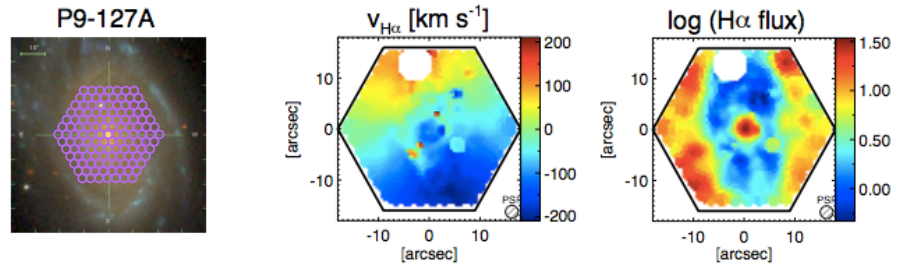
\includegraphics[width=0.95\textwidth]{discussion/manga_data.png}}
\caption[Example MaNGA fibre bundle on a target galaxy with example emission data]{Example fibre bundle placed over a MaNGA target galaxy (left) and corresponding preliminary survey data showing the mapped velocity (middle) and flux (right) of $H\alpha$ gas emission as measured across the galaxy in each fibre. Such measurements can be utilised to calculate the star formation rate across the structure of a galaxy. Adapted from \cite{bundy15} Figure 14.}
\label{fig:manga}
\end{figure}

In Chapter \ref{chap:agn} I discussed how the current SDSS data (both photometric and spectroscopic) cannot determine whether the AGN is the cause or the consequence of the quenching seen across the AGN host population in Figures \ref{time} \& \ref{rate}. Using data from the MaNGA IFU survey \citep{bundy15} I hope to determine whether feedback from the AGN is truly the cause of this quenching. The MaNGA survey will provide 127 spectra across a single galaxy (see Figure~\ref{fig:manga}), allowing the SFH to be mapped as a function of radius. The acquisition of a spectrum in each of these apertures allows for the modification of \starpy\ to take spectral star formation indicators \citep[such as $H\alpha$][]{kennicutt94} to break the degeneracy provided by the photometric colours (see Figure~\ref{pred}), and also the easy removal of any unobscured AGN in the central regions. 

Any correlation of the inferred quenching parameters with radius of the galaxy will allow the determination of whether quenching is happening from the outside-in \citep[i.e. due to the environment, as in][]{pan15, clarke16, schaefer17} or inside-out, as in work with preliminary MaNGA survey data by \citet{belfiore16} and with CALIFA data by \citet{gonzalez16}. I will investigate how this preference for outside-in or inside-out quenching is correlated with the presence of an AGN and a galaxy's environment. This will no only help to answer the question of \emph{cause} vs. \emph{consequence} but also further constrain the timescales of quenching mechanisms possibly caused by AGN or environment. 

\section{Hubble Space Telescope follow up}\label{sec:hst}

In Chapter~\ref{chap:agn}, I discussed how accurate fits to the bulge-to-total ratio could not be made for galaxies of the \textsc{bulgeless} sample hosting AGN due to the resolution of ground based SDSS imaging. This led to the derivation of upper limits on the bulge masses of this sample. The Hubble Space Telescope (HST) however, provides (i) an extremely stable and well understood point spread function, enabling reliable separation of the AGN from the host galaxy, and (ii) high spatial resolution which is needed to distinguish between classical, merger driven bulges and pseudo bulges grown by secular processes. Observations with the HST of the galaxies in the \textsc{bulgeless} sample will enable extremely robust measures of bulge-to-total ratios for each host galaxy and allow the identification of truly secular systems with growing black holes. Such measurements will also allow the interplay between merger driven (building classical bulges) and merger free (growing pseudo-bulges or retaining a pure disc) co-evolutionary histories to be disentangled. 

\begin{figure*}
\centering{
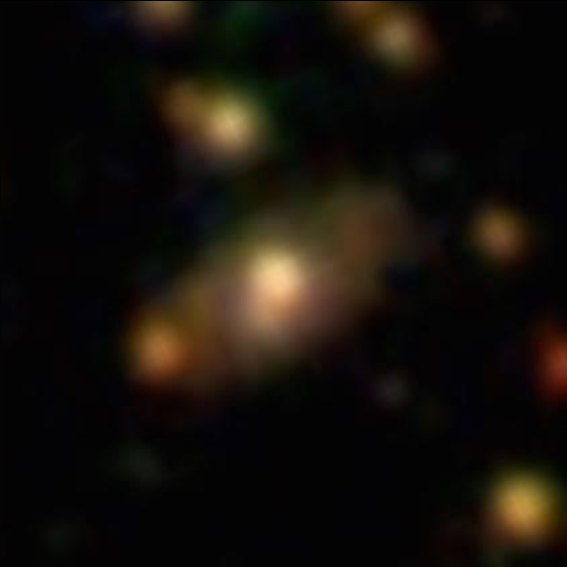
\includegraphics[width=0.49\textwidth]{discussion/sdss_data.png}
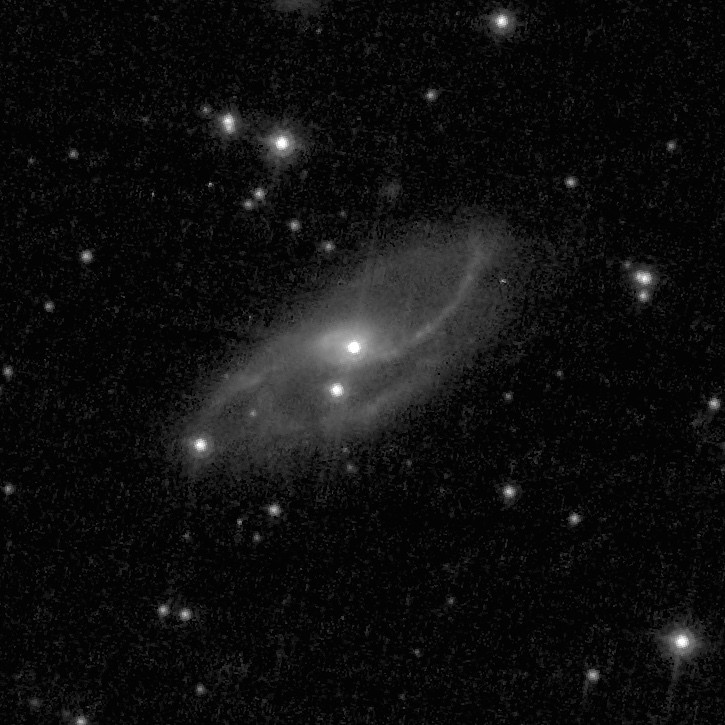
\includegraphics[width=0.49\textwidth]{discussion/hst_data.jpg}}
\caption[Example HST image data in comparison to SDSS]{Example SDSS urgiz image (left) for J$192250.74$-$055259.15$, part of the \textsc{bulgeless} sample, described in Section~\ref{sec:selectAGN}, in comparison to space based imaging from the HST (right). The higher resolution HST image reveals finer structure than the SDSS image, including spiral arms, a ring and a possible bar along with the true disc dominated nature of the galaxy.}
\label{fig:hstdata}
\end{figure*}

Figure~\ref{fig:hstdata} demonstrates the difference in resolution provided by the HST with some of the first data received from our successful proposal (ID: 14606, Cycle 24) to observe galaxies in the \textsc{bulgeless} sample. The galaxy shown is J$192250.74$-$055259.15$ in comparison with the ground based SDSS ugriz image (left; also shown in Figure~\ref{fig:INTimages}). This galaxy has an estimated black hole mass of $M_{\rm{BH}} = 10^{7.4\pm0.1}~M_{\odot}$ but a bulge-to-total ratio could not be derived from the SDSS image. The HST image will allow for an accurate derivation of the bulge mass of this galaxy, allowing for a more concrete conclusion to be drawn on the controversial issue of secularly driven galaxy-black hole co-evolution. 

